\subsection{HCAL Calibrations}

The calibration of the hadron calorimeter\footnote{Details of the detector are presented in \ref{CMS}} (HCAL) is vital in the determination of the energy scale and resolution of hadrons, and consequently jets and missing transverse momentum.

There are no HCAL calibrations included in the PCL, however, there exist HCAL automation workflows that update HCAL conditions on a weekly basis (e.g. gains, pedestals). Most conditions are explicitly baked into the Look-Up Tables (LUTs) that are loaded on-detector and append the GT via the O2O procedure semi-automatically. The remaining conditions are uploaded manually to the conditions database. Many HCAL conditions are also relevant for L1T and the corresponding trigger primitives. Out of the 326 conditions in the HLT GT, 37 are related to HCAL, of which 24 are relevant to Run 3 data-taking. From these, the following 9 are considered core and critical for data-taking:

\begin{table}[h!]
    \centering
    \begin{adjustbox}{max width=\textwidth}
    \begin{tabular}{p{3.5cm}|p{4cm}|p{2.5cm}|p{2cm}|p{4.5cm}}
        \textbf{Name} & \textbf{Record} & \textbf{Workflow} & \textbf{Frequency of Updates} & \textbf{Description} \\ \hline
        Gains (RadDam) & \texttt{HcalGains} & O2O & Weekly & Response corrections for radiation damage (RadDam). \\
         Pedestals & \texttt{HcalPedestals} & HCAL automation (O2O) & Weekly & Pedestals for noise measurements.
measurements.\\
        Pedestal Widths & \texttt{HcalPedestalWidths} & HCAL automation (O2O) & Weekly & Pedestals for noise measurements.
measurements. \\
        L1T Trigger Objects & \texttt{HcalL1TriggerObjects} & HCAL automation (O2O) & Weekly & L1T trigger objects, including relevant conditions: pedestals, gains and response corrections, channel quality. \\
        Response Corrections & \texttt{HcalRespCorrs} & O2O & per Era ($\approx 20~\fbinv$) & Corrections to detector energy response. \\
        Channel Quality & \texttt{HcalChannelQuality} & O2O & Few times per year & Tracking dead or non-functional HCAL cells. \\
        Geometry Parameters & \texttt{HcalParameters} & Manual & Yearly & Parameters related to the HCAL geometry. \\
        Look-Up Tables (LUTs) & \texttt{HcalLUTCorrs} & O2O & Rarely & Corrections related to Look-Up Tables (LUTs). \\
    \end{tabular}
    \end{adjustbox}
    \caption{Fundamental HCAL Calibrations, ordered in terms of frequency of updates.}
    \label{tab:HCALCalibrations_critical}
\end{table}

In the context of an optimal calibrations workflow, the first 6 from Table \ref{tab:HCALCalibrations_critical} are considered fundamental\footnote{There exist fundamental HCAL conditions or calibrations which can have a significant effect on HLT reconstruction that are implemented in the hardware directly (e.g. timing alignment, zero-suppression thresholds, \texttt{HcalZSThresholds}) while their conditions database records may not be considered critical per se (but rather used for bookkeeping purposes).} and generally require more frequent updates. These have been analysed in more detail in the following sections. % NOTE: footnote could be moved to Others section.

\subsubsection{Response Corrections}
Response corrections are calibrations that aim to equalise the signal coming from the detector to provide a uniform energy measurement. They have a very significant effect on HLT reconstruction and rates, and thus are considered critical. Generally, they are updated roughly every era ($\approx 20 \fbinv$), however, the exact frequency depends on the HCAL subsystem and type of correction. Generally, the required statistics determines the frequency, as the analyses are often statistically limited. Technically-speaking, if the calibrations are determined accurately, they would require less-frequent updates (modulo hardware changes). The updates are explicitly baked into the LUTs that are loaded on-detector and the corresponding conditions appended to HLT GT via the O2O procedure semi-automatically.

% HB and HE
The main calibrations for the HB and HE come in in two forms: azimuthal ($\phi$\texttt{-symmetry}) and isolated track (\texttt{IsoTrack}) corrections, which are multiplicative factors. 

% Azimuthal (Phi-)Symmetry
Asymmetries in the response over $\phi$ arise due to structure, materials, inhomogeneous magnetic field, beam-spot shifts, and miscalibrations. The $\phi$\texttt{-symmetry} intercalibrations equalize the detector response in $\phi$ for each $i\eta$ ring and depth section of the HCAL. They take advantage of the uniformity of particle energies across the azimuthal angle $\phi$. An intercalibration is performed between calorimeter channels by comparing it to the average collected energy in the entire $i\eta$ ring. Two methods are used to determine them, depending on the hadron energies:
\begin{itemize}
    \item For high energies ($> 4 \GeV$) an iterative method is used, where scale factors for uncalibrated energies are determined iteratively by equalizing the mean of the energies in an energy interval. An unbiased dataset is used with events triggered by detectors other than HCAL, such as electron, photon and muon triggers. The reconstructed energies are obtained from zero-suppressed events after noise (pedestal) subtraction.
    \item For low energies ($< 4 \GeV$; down to a fraction of a GeV), a method of moments is used, where the first (mean) and second (variance) moments of the energy distribution are compared to that of the entire $i\eta$ ring. This method uses minimum-bias events taken without zero-suppression (NZS). The noise (pedestal) is subtracted from the energy distribution.
\end{itemize}

The uncertainty-weighted average of the scale factors from both methods is used as the final scale factor for the $\phi$-intercalibration.

% Isolated Track (IsoTrack)
An absolute calibration of charged hadrons is performed by comparing the energy measurement with that of the tracker system, taking advantage of the precise calibration of the tracker system. Unlike the tracker momentum measurement, the HCAL energy response is non-linear, especially at lower energies. Therefore, the goal of the calibration is to equalize the relative energy scale for higher momentum charged hadrons that do not interact hadronically with the ECAL. Isolated tracks of hadrons with momenta between $40-60 \GeV$ are used. Data samples are collected using dedicated \texttt{IsoTrack} triggers with special isolation and maximum requirements on the energy deposited in the ECAL, as well as a more standard set of physics triggers with similar selections applied offline. Assuming there are no statistical limitations, preferably they are determined in a depth-dependent way, which is more optimal.

% HF
The forward calorimeter (HF) is also calibrated using the $\phi$-symmetry, while the energy scale is extrapolated using $Z \rightarrow ee$ events. The dataset consists of events with one electron candidate in the HF and the other in the ECAL, which has been precisely calibrated. The scale is adjusted so that the dielectron invariant mass corresponding to the Z-peak is consistent between data and simulation.

% HO, ZDC
For HO, the intercalibration makes use of muons from collision data, as well as cosmic ray muons, while the determination of the absolute energy scale makes use of di-jet events. These calibrations are mostly unchanged with respect to initial calibrations.

The Zero-Degree Calorimeter (ZDC) calibrations are also mostly unchanged and are not discussed here further. 

% NGT candidate assessment
In the context of a potential candidate for the optimal NGT calibrations, it is clear that the response corrections involve a number of dedicated separate offline analyses for different HCAL subsystems, using various input datasets (incl. \texttt{AlCaRecos}) and specific selections. Thus, their determination is rather convoluted and they are tricky to do without proper offline analysis and corresponding validation. Even though some of the sub-calibrations might be reasonably possible to automate (e.g. $Z \rightarrow ee$ for HF), it would still require significant work to automate. Furthermore, since they are baked into the LUTs, they are entangled together with L1T condition updates. Therefore, one can conclude that the response corrections are not a viable candidate for the NGT workflow in their current form, especially for the Run 3 prototype.

\subsubsection{Gains (RadDam)}\label{sec:HCAL_gains}
The  \textit{gains} (or \texttt{RadDam}) calibrations are responsible for correcting for radiation damage in the HCAL. Generally this leads to a decreased signal due to the darkening of active scintillator material and fibres (similar to the ECAL laser corrections covered in Section \ref{sec:ECALlaser}). Conversely, the recovery process of thermal annealing also effects the signal and needs to be corrected for. Due to the increased radiation in the forward region, primarily HE and HF are corrected. These corrections are especially important in the high $|i\eta|$ regions where there is no tracker coverage and the \texttt{IsoTrack} response corrections are less accurate and cannot cover for these differences. Therefore, they can be considered critical especially for those regions. HB and HO have not been corrected for a long time due to lower radiation damage. The corrections are determined $|i\eta|$- and depth-dependent and $|i\phi|$-independent) yielding a multiplicative factor together with the response corrections for final calibrated response in GeV. Generally, they are updated via the O2O procedure semi-automatically (as with the response corrections) roughly every era ($\approx 20 \fbinv$).

Typically, the measurements of the radiation damage is based on laser data in the orbit/abort gap, when there is no beam in the LHC. The laser system sends light to the photodetectors (SiPMs, PMTs) or directly to the scintillators. The ratio of the amplitudes gives a measure of the signal attenuation. The laser data is then compared to that taken at the start of the yearly data-taking in order to measure the net effects of radiation damage. A new dedicated radiation damage monitoring system was recently developed for the HF quartz fibres. 

The effects of radiation damage are dependent on the delivered luminosity. The dependence is modelled and parametrised to exponential decay \cite{CMS-PRF-18-003}. An example of the relative laser signal in a single $i\eta$ region and layer is shown in Figure \ref{fig:ECAL-Laser_data}. 

\begin{figure}[h!]	
\centering
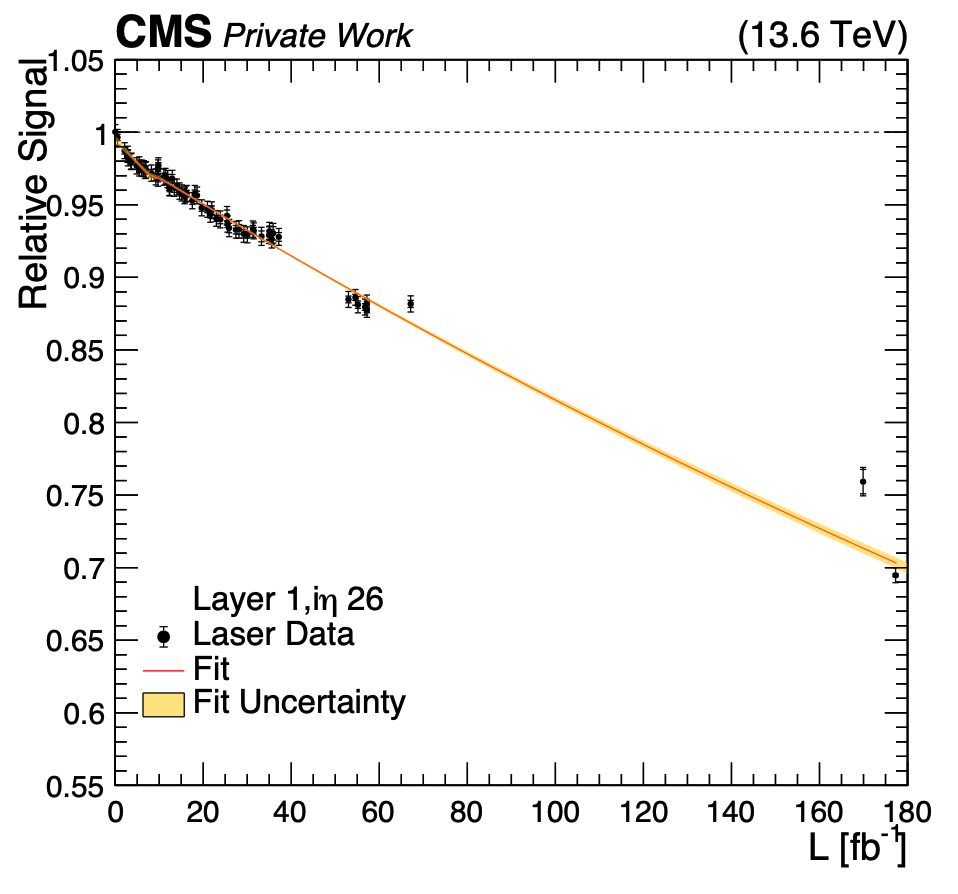
\includegraphics[width=0.7\textwidth]{figures/HCAL-Laser_data2024.png} %\hfill
\caption{Laser system data in layer 1, $i\eta = 27$ of the HCAL, indicating the relative signal as a function of the total integrated luminosity L in $\fbinv$, parametrised as exponential decay. The missing data points indicate the extended downtime of the laser system in 2024.}
\label{fig:HCAL-Laser_data}
\end{figure}

In the case of downtime of the laser system (also seen in Figure \ref{fig:ECAL-Laser_data} for 2024), the backup approach are dedicated energy flow extrapolations, which are non-trivial. Therefore, the preference is to use laser data.

% NGT candidate assessment
In the context of a potential candidate for the optimal NGT calibrations, the gains or \texttt{RadDam} corrections are important for HLT reconstruction and require frequent updates. There are plans to include them in the HCAL automation system (covered in more details the next Section \ref{sec:HCAL_pedestals}) within weekly updates. Therefore, they are a good candidate for the NGT workflow. One caveat is that they are dependent on laser data, which requires a different data stream than the standard bulk collisions data. Furthermore, a vital requirement is a well-functioning laser system.

\subsubsection{Pedestals}\label{sec:HCAL_pedestals}
The HCAL pedestals and their corresponding widths are essentially measurements of the noise "floor" that are offset to avoid any energy measurement bias. Generally, noise increases with radiation damage. Regular pedestal updates are important to avoid any drifting of HCAL-driven trigger rates and contributions to the fraction of the energy deposited in the HCAL and ECAL, $\frac{H}{E}$, which is an observable used in the identification of electrons and photons, including shower shapes and isolation. The pedestals are also important inputs into other calibrations, such as the response corrections.

Generally, they are updated roughly every week ($\approx 2 \fbinv$), as part of the HCAL automation workflow. The workflow, based on Jenkins, is used to calculate effective pedestals from collision runs, where good input data from candidate runs is identified and processed within 1 hour after a given LHC fill. The input data is based on measurements in orbit/abort gap when there is no beam in the LHC (similarly to the laser data for the HCAL gains discussed in the previous Section \ref{sec:HCAL_gains}). The conditions are then automatically uploaded to the conditions database via the O2O procedure. Validation in the context of changes to L1T and HLT trigger rates are produced within 2 hours, with an ultimate validation and green-light from AlCa typically after 1-2 days. Given a successful validation, this is followed by deployment at the subsequent LHC interfill period.

% NGT candidate assessment
In the context of a potential candidate for the optimal NGT calibrations, the pedestals are critical inputs. They are included in the HCAL automation system within weekly updates, which automatically make them a good candidate for the NGT workflow. One caveat is that they are dependent on orbit/abort gap data, which requires a different data stream than the standard bulk collisions data.

% \subsubsection{Others}

% NOTE: more complete list in annex? e.g. non-critical calibrations